% Withdrawn analyses removed from the appendix for the ICLR 2027 rebuttal revision.
% Not compiled. Kept for the supplementary record; ERRATA.md summarises every changed claim.

\section{Linear Probing: Functional Representation Diagnostic}
\label{app:probing}

\noindent\fbox{\parbox{0.97\linewidth}{\textbf{Retracted.} The analyses in this
appendix rest on the linear-probe $\Delta R^2$ statistic, which is retracted
(\S\ref{sec:retraction}): it is non-zero only where the probe fails to
generalise. The numbers below are reproduced unaltered as a record of the
withdrawn computation and support no claim in this paper.}}
\vspace{1em}
% ============================================================

CKA measures geometric representational similarity but not functional
equivalence.  We therefore supplement CKA with a \emph{linear probe}:
a Ridge regression head ($\alpha{=}1.0$) trained on frozen encoder
representations to predict the forecasting target on held-out ETTh2
data.

\textbf{Protocol.}
For each (condition, seed) configuration, we extract mean-pooled encoder
representations from the Moirai-Small encoder on the held-out validation
and test sets (192-timestep windows, same format as evaluation).
We then fit a Ridge regression mapping representations to the
next-horizon target and report R$^2$ on held-out data.
The probe training set uses $n_{\text{probe}}{=}300$ held-out examples;
the remainder forms the test split used for MSE evaluation.
$\Delta R^2$ denotes fine-tuned minus pre-trained probe R$^2$:
positive values indicate that fine-tuned representations encode
more forecasting-relevant information than pre-trained ones.

\textbf{Interpretation.}
Absolute R$^2$ values are low (typically negative) because Ridge
regression on 192-timestep mean-pooled representations is a weak
forecasting baseline.  The \emph{relative} change ($\Delta R^2$)
is the meaningful signal: it isolates whether fine-tuning added
or removed task-relevant information from the encoder's
representational basis.

\textbf{Key result.}
Across the sample-size sweep (the transcript in \S\ref{sec:retraction};
Table~\ref{tab:sample_sweep} no longer prints these columns)
$\Delta R^2$ increased monotonically with training data
(Ridge: $+$0.12 at 500 samples $\rightarrow$ $+$0.67$\pm$0.24
at 10{,}000 on CUDA 10-seed deterministic early-stopped encoders,
\texttt{results/v19\_cuda\_etth2\_n10k/}; for comparison, MPS early-stopped
$k{=}5$ gave $+$0.56$\pm$0.14 (\texttt{v17\_etth2\_n10k\_es}) and the
final-epoch runs, $k{=}3$, gave $+$0.84$\pm$0.15
(\texttt{v16\_etth2\_n10k})), while CKA decreases monotonically.
This directly dissociates \emph{geometric} drift from
\emph{relative linear-decodability}: at low $n$, drift destroys
task-relevant features faster than it builds replacements;
at higher $n$, the fine-tuned representation becomes less
linearly misaligned with the forecasting target than the
pre-trained one.
We emphasise that $R^2(\text{FT})$ remains
\emph{absolutely negative} at every sampled
$n \in \{500, 1\text{k}, 2\text{k}, 5\text{k}, 10\text{k}\}$
(ZS: $R^2{=}-6.90$; CUDA $k{=}10$ early-stopped: $-6.79$ at $n{=}500 \to -6.24{\pm}0.24$
at $n{=}10$k).  $\Delta R^2 {>} 0$ is therefore a
\emph{relative-improvement} signal, not a claim that
fine-tuned representations linearly encode the target well
in absolute terms; the primary task-outcome signal remains
forg.$<0$ at $n{\geq}2$k.
\textbf{Cross-dataset $\Delta R^2$ comparability.}
Raw $\Delta R^2$ is not directly comparable across datasets because
it depends on the ZS Ridge floor depth.
On ETTm2 ($n{=}10$k, CUDA, $k{=}5$), the ZS Ridge floor is
$R^2(\text{ZS}){=}-24.52$, 3.5$\times$ deeper than ETTh2's
$-6.90$, which proportionally inflates the raw $\Delta R^2$
($+$6.35 on ETTm2 vs.\ $+$0.67 on ETTh2).
The cross-dataset comparable statistic is the \emph{sign test}: ETTh2 gives
\textbf{10/10} positive $\Delta R^2$ and ETTm2 \textbf{5/5}, on the five CUDA
seeds that exist for that cell.  Every dispersion in this appendix is a standard
deviation over seeds at $\text{ddof}{=}1$.

\textbf{Horizon-sweep probe: head-specificity of the $\Delta R^2$ gain.}
Table~\ref{tab:probe_horizon} reports Ridge $\Delta R^2$ across three
probe heads on four early-stopped encoders at $n{=}10$k (the
same encoders as the main-text MLP sweep).  The gain is concentrated
on the \emph{trained} 96-step head: $\Delta R^2{=}{+}0.116{\pm}0.153$
($k{=}4$).  On the untrained \emph{forecast48} head (first 48 steps
of the 96-step target, a sub-horizon the encoder was not directly
optimised for), $\Delta R^2 {=} {-}0.001{\pm}0.163$: the gain
vanishes at the horizon boundary.  On the untrained \emph{delta1}
head, a GBM probe gives $R^2(\text{PT}){=}{+}0.059{>}0$, establishing
a positive-floor reference, with $\Delta R^2{=}{-}0.056{\pm}0.032$
(decodability \emph{falls} on the untrained readout).
The head-specificity pattern is consistent with the encoder drifting
toward the fine-tuning objective rather than developing generally
better representations (Table~\ref{tab:r2task}).

\begin{table}[ht]
\centering
\caption{Ridge $\Delta R^2$ by probe head on early-stopped encoders ($n{=}10$k,
seeds \{303, 777, 888, 999\}).  ``Forecast96'' is the trained head;
``Forecast48'' and ``Delta1'' are untrained.  The gain is head-specific
to the trained objective.  Every entry is
$R^2(\text{FT}){-}R^2(\text{ZS})$ read from
\texttt{results/v18\_reprobe/seed*\_horizons.json} against
\texttt{zs\_horizons.json}; dispersion is the standard deviation over the four
seeds ($\text{ddof}{=}1$).}
\label{tab:probe_horizon}
\small
\begin{tabular}{lccccc}
\toprule
Head & Trained? & \multicolumn{4}{c}{Ridge $\Delta R^2$ per seed} \\
& & s303 & s777 & s888 & s999 \\
\midrule
Forecast96 (96-step ahead) & \checkmark & $+$0.092 & $-$0.087 & $+$0.266 & $+$0.192 \\
Forecast48 (sub-horizon) & $\times$ & $+$0.061 & $-$0.111 & $-$0.156 & $+$0.199 \\
Delta1 (next-step delta) & $\times$$^\dagger$ & $+$1.248 & $+$0.757 & $+$1.191 & $+$0.980 \\
\midrule
\multicolumn{2}{l}{Mean $\pm$ std (forecast96)} & \multicolumn{4}{c}{$+$0.116 $\pm$ 0.153} \\
\multicolumn{2}{l}{Mean $\pm$ std (forecast48)} & \multicolumn{4}{c}{$-$0.001 $\pm$ 0.163} \\
\multicolumn{2}{l}{Mean $\pm$ std (delta1)} & \multicolumn{4}{c}{$+$1.044 $\pm$ 0.223} \\
\bottomrule
\end{tabular}
\vspace{2pt}
{\small $^\dagger$\,The large Ridge $\Delta R^2{>}0$ on Delta1 reflects a
baseline-floor artifact: $R^2(\text{ZS})$ is deeply negative on the next-step
target, so any encoder shift appears to improve relative decoding.
A gradient-boosted probe gives $R^2(\text{PT}){=}{+}0.059$ (positive floor)
but $\Delta R^2{=}{-}0.056{\pm}0.032$ on this head
(\texttt{results/v18\_reprobe/seed*\_delta1.json}), consistent with the shift
\emph{not} being aligned with the 1-step objective.}
\end{table}

Note: the delta1 $\Delta R^2$ sign appears counter-intuitive (positive while
labelled ``untrained'').  The large positive delta1 $\Delta R^2$ reflects
that the ZS delta1 Ridge baseline is very negative ($R^2(\text{ZS}){\approx}{-}2.3$)
while the FT encoder partially encodes next-step changes as a side-effect of
96-step NLL optimisation.  The diagnostic signal is the GBM result
(Table~\ref{tab:r2task}): GBM gives $R^2(\text{PT}){=}{+}0.059{>}0$
and $\Delta R^2{=}{-}0.056$, yielding $R^2(\text{FT}){=}{+}0.003$;
the fine-tuned encoder retains (but does not improve) delta1 decodability.
With a positive floor, decodability \emph{falls} on the untrained readout,
confirming task-alignment.
Note: $R^2(\text{PT})$ varies slightly across GBM probe depths
(depth~4: $+$0.062, depth~6: $+$0.059, depth~8: $+$0.054;
\texttt{results/v20\_gbm\_sensitivity/}) because the probe is re-fit
independently at each depth; this reflects probe capacity, not encoder
structure.  $\Delta R^2$ keeps its sign at all three depths
($-0.060{\pm}0.006$, $-0.056{\pm}0.032$, $-0.052{\pm}0.006$).

\textbf{ETTm2 delta1 GBM reprobe.}
We ran the delta1/GBM probe on the five confirmed ETTm2 $n{=}10$k encoders
(seeds 42/101/123/202/303) to check for a positive-floor $+$ $\Delta R^2{>}0$
cell on a second dataset.
Result: $R^2(\text{ZS}){=}{-}0.030$ (negative floor) and per-seed
$\Delta R^2{=}\{+0.025, -0.060, +0.026, +0.030, +0.016\}$ in seed order
(4/5 positive, mean $+0.007{\pm}0.038$;
\texttt{results/v25\_ettm2\_delta1\_gbm/}).  \emph{Substantive negative:} the
only positive-floor head (ETTh2 delta1/GBM, $R^2(\text{ZS}){=}{+}0.059$) gives
$\Delta R^2{=}{-}0.056$; no positive-floor $+$ $\Delta R^2{>}0$ cell was found.
The $\Delta R^2{>}0$ signal on the trained 96-step head operates in a
deeply-negative-$R^2$ regime; see Appendix~\ref{app:noisefloor} for probe
noise-floor analysis.

\textbf{Per-seed breakdown at $n{=}10$k (CUDA 10-seed).}
Ridge $\Delta R^2$ (all positive; mean $+0.668{\pm}0.239$,
\texttt{results/v19\_cuda\_etth2\_n10k/}):
42:$+0.205$; 101:$+0.736$; 123:$+0.937$; 202:$+0.604$; 303:$+0.793$;
456:$+0.823$; 777:$+0.344$; 789:$+0.873$; 888:$+0.561$; 999:$+0.804$.
Absolute $R^2(\text{FT})$: all in $[-6.70, -5.97]$ ($R^2_{\text{ZS}}{=}-6.904$).
MLP $k{=}5$ (all positive; mean $+0.701{\pm}0.324$):
42:$+0.979$; 101:$+0.762$; 123:$+0.948$; 202:$+0.771$; 303:$+1.007$;
456:$+0.266$; 777:$+0.076$; 789:$+0.847$; 888:$+0.449$; 999:$+0.901$.

\textbf{ETTm2 $n{=}10$k absolute $R^2$ per seed.}
The ETTm2 ZS Ridge floor ($R^2(\text{ZS}){=}-24.52$, same pre-trained
encoder across all seeds) is 3.5$\times$ deeper than ETTh2's $-6.90$,
explaining the raw $\Delta R^2$ magnitude difference.
Per-seed absolute values for the five available CUDA seeds:

\begin{center}
\small
\begin{tabular}{lcccc}
\toprule
Seed & $R^2$(ZS) & $R^2$(FT) & $\Delta R^2$ & Forg.\% \\
\midrule
42  & $-24.52$ & $-14.13$ & $+10.39$ & $-26.8$ \\
101 & $-24.52$ & $-15.61$ & $+8.91$  & $-27.4$ \\
123 & $-24.52$ & $-19.87$ & $+4.64$  & $-31.1$ \\
202 & $-24.52$ & $-20.83$ & $+3.69$  & $-28.8$ \\
303 & $-24.52$ & $-20.41$ & $+4.11$  & $-29.5$ \\
\midrule
Mean (5 seeds) & $-24.52$ & $-18.17{\pm}3.08$ & $+6.35{\pm}3.08$ & $-28.7{\pm}1.6$ \\
\bottomrule
\end{tabular}
\end{center}

All five seeds show $R^2(\text{FT}) > R^2(\text{ZS})$ (i.e., fine-tuned
representations are \emph{less} linearly misaligned with the ETTm2
forecasting target than pre-trained ones), and all show $\Delta R^2{>}0$.
The cross-dataset comparable statistic is the sign test: ETTh2 gives
\textbf{10/10} on seeds 42, 101, 123, 202, 303, 456, 777, 789, 888, 999 and
ETTm2 \textbf{5/5} on 42, 101, 123, 202, 303, the only five CUDA $n{=}10$k
encoders that exist for ETTm2 (\texttt{results/v19\_cuda\_ettm2\_n10k/}).

\textbf{MLP depth sweep on early-stopped encoders.}
A cosine-LR re-run at $n{=}10$k uses seeds
$\{303, 777, 888, 999\}$ at $\mathrm{epochs}{=}10$ (seed 101
MPS-NaN'd on epoch~3 reproducibly at this schedule and is excluded).
The \texttt{--probe-mlp-layers}
argument sweeps hidden-layer depth $k \in \{1, 2, 5\}$ on the
early-stopped encoders (probe: hidden=64 per layer, $\alpha{=}10^{-3}$,
early stopping with validation\_fraction=0.1, max\_iter=500).  All sixteen
entries below are read from
\texttt{results/v17r2\_etth2\_n10k\_es\_mlp/seed*/}, and its Ridge column is the
same one Table~\ref{tab:probe_horizon} reports as \emph{forecast96}: the two
tables re-probe one set of encoders, they are not two runs.

\begin{center}
\begin{tabular}{c c c c c}
\toprule
Seed & Ridge $\Delta R^2$ & MLP $k{=}1$ & MLP $k{=}2$ & MLP $k{=}5$ \\
\midrule
303 & $+0.092$ & $+1.306$ & $+1.418$ & $+0.540$ \\
777 & $-0.087$ & $+1.136$ & $+1.554$ & $+0.759$ \\
888 & $+0.266$ & $+2.004$ & $+2.361$ & $+1.034$ \\
999 & $+0.192$ & $+1.816$ & $+1.949$ & $+0.908$ \\
\midrule
Mean $\pm$ std & $+0.116{\pm}0.153$ & $+1.566{\pm}0.411$ & $+1.821{\pm}0.425$ & $+0.810{\pm}0.212$ \\
\bottomrule
\end{tabular}
\end{center}

The cosine-LR Ridge $\Delta R^2$ is smaller than the epochs=20 run
($+0.56{\pm}0.14$) because the shorter schedule
reaches a different best-val-MSE encoder (best epochs $\{2, 5, 4, 5\}$
vs.\ $\{2, 4, 8, 4, 3\}$), and Ridge is most sensitive to the
specific linear basis.  The non-monotonic $k{=}1 \to k{=}2 \to k{=}5$
trend reflects the deeper probe fitting the pre-trained encoder
better (per-seed mean $R^2(\text{PT})_{k{=}5}{=}-6.93$ vs.\
$R^2(\text{PT})_{k{=}1}{=}-8.48$), shrinking the $\Delta$ from
above, not degraded fine-tuned encoding.  All four seeds
are individually positive for $k{=}5$ MLP
($+0.54, +0.76, +1.03, +0.91$), preserving the cost--benefit gap.
This run's CKA is $0.592{\pm}0.164$ (mean best epoch
$4.0{\pm}1.41$, earlier than the epochs=20 run's $4.2{\pm}2.3$ because of the
earlier LR annealing);
forgetting is $-7.13{\pm}1.55\%$, tighter than the epochs=20 run's
$-11.7{\pm}5.3\%$ and fully consistent with the forg.$<0$ finding.

\textbf{Crossover regime: per-seed breakdown at $n{=}5{,}000$.}
Table~\ref{tab:n5k_seeds} reports all 7 seeds individually at
$n{=}5{,}000$.  Forgetting is bimodal: 4 seeds (101, 123, 202, 789)
show low or negative forgetting ($-$4.9\% to $+$5.9\%, mean $+0.7$\%)
and 3 seeds (42, 303, 456) show high forgetting ($+$4.8\% to $+$21.4\%,
mean $+15.1$\%).
All 7 seeds show positive $\Delta R^2$ ($+$0.15 to $+$0.81, mean $+$0.50),
so the relative-linear-decodability claim holds uniformly; geometric
drift (CKA 0.46--0.71, mean 0.55) varies less than forgetting.
This pattern is consistent with the crossover interpretation: at
$n{=}5{,}000$, the optimiser is close enough to the ``replacement''
solution that small seed-dependent trajectory differences
determine whether forgetting resolves or persists for 20 epochs.

\begin{table}[t]
\centering
\caption{Per-seed results at $n{=}5{,}000$ (ETTh2, $h{=}96$, condition B,
20 epochs, no early stopping).  Seeds 42, 123, 456 are the original 3-seed sweep
(\texttt{results/v8\_final/n5000/}); 789, 101, 202, 303 are the 4-seed V9
replication (\texttt{results/v9\_n5k\_seeds/}).  MSE(FT) is
\texttt{final\_val\_mse}, the last-epoch validation MSE, and was previously
printed 2--5 thousandths low on every row.  Forgetting is bimodal; $\Delta R^2$
is uniformly positive.}
\label{tab:n5k_seeds}
\small
\begin{tabular}{rccccc}
\toprule
Seed & MSE(FT) & Forg.\% & CKA & $\Delta R^2$ & R$^2$(FT) \\
\midrule
 42  & .136 & $+$4.8  & .531 & $+$.67 & $-$6.24 \\
101  & .121 & $-$4.9  & .571 & $+$.75 & $-$6.16 \\
123  & .129 & $-$1.4  & .544 & $+$.81 & $-$6.10 \\
202  & .131 & $+$1.4  & .461 & $+$.15 & $-$6.76 \\
303  & .152 & $+$19.0 & .525 & $+$.52 & $-$6.39 \\
456  & .155 & $+$21.4 & .711 & $+$.20 & $-$6.70 \\
789  & .136 & $+$5.9  & .480 & $+$.40 & $-$6.51 \\
\midrule
Mean$\pm$std & .137$\pm$.012 & $+$6.6$\pm$10.0 & .546$\pm$.082 & $+$.50$\pm$.26 & $-$6.41$\pm$.26 \\
\bottomrule
\end{tabular}
\end{table}

\subsection{$n{=}5{,}000$ per-epoch trajectory analysis}
\label{app:n5k_trajectories}

To support the mechanistic claim in \S\ref{sec:exp3}, we plot the
per-epoch training trajectories of all seven $n{=}5{,}000$ seeds,
colour-coded by forgetting mode.  Figure~\ref{fig:n5k_trajectories}
shows val MSE and weight drift across training.  High-forgetting seeds
(303, 456, 789) overshoot in the first epoch and never recover;
low-forgetting seeds (42, 101, 123, 202) continue descending until
epochs 3--8.  The epoch at which val MSE reaches its minimum separates
the modes ($0.7\pm0.5$ vs.\ $6.5\pm2.1$); mid-training weight drift
(epochs 5--10) does not.  Code: \texttt{scripts/analyse\_n5k\_trajectories.py}.

\begin{figure}[t]
\centering
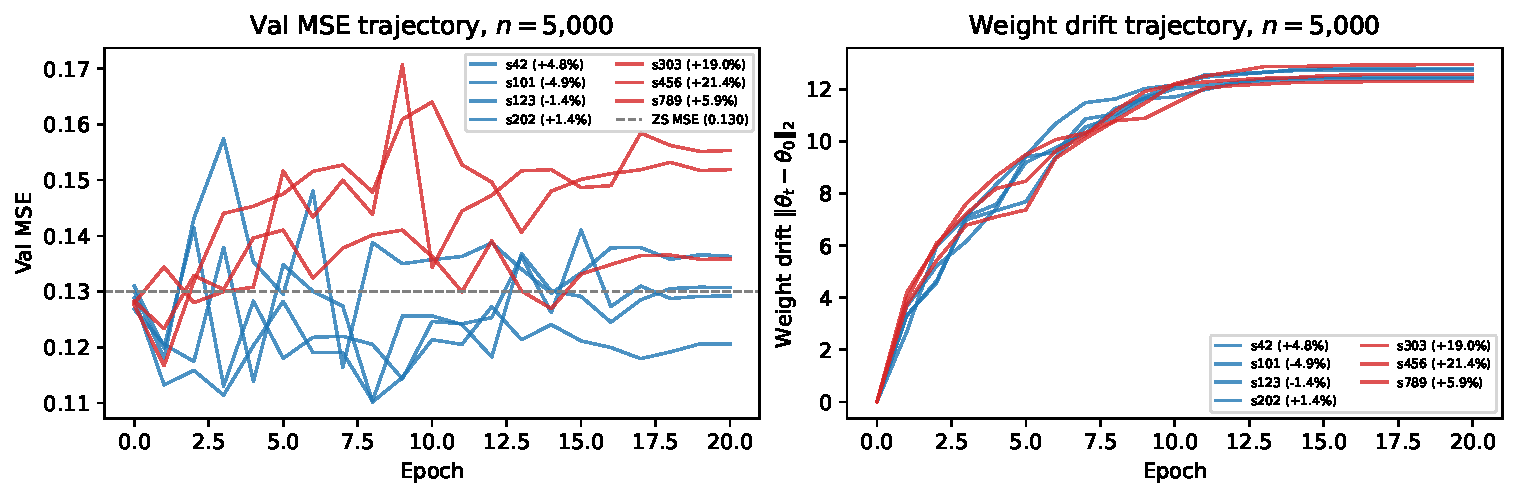
\includegraphics[width=\linewidth]{figures/n5k_trajectories.pdf}
\caption{Per-epoch val MSE (left) and weight drift (right) for the
seven $n{=}5{,}000$ seeds; both panels carry per-seed labels
(\texttt{sXXX (forg.\%)}) so each trajectory is individually
identifiable. Blue: low-forgetting mode (forg.~$\le$~5\%);
red: high-forgetting mode (forg.~$>$~5\%). Grey dashed line: zero-shot
MSE. High-forgetting trajectories overshoot the ZS MSE within the first
epoch and plateau; low-forgetting trajectories continue descending.
Mid-training weight drift (epochs 5--10) does not separate the modes.}
\label{fig:n5k_trajectories}
\end{figure}

% ============================================================
\section{ETTh1 Spectral Pilot}
\label{app:etth1_extended}
% ============================================================

Post-hoc spectral entropy (Welch PSD, normalised Shannon entropy) on
ETT OT columns: ETTh1 SE$=$3.61~bits, ETTh2 SE$=$3.46, ETTm2 SE$=$2.25.
The ordering this pilot was built to explain was an ordering of
$\Delta R^2$, which is \textbf{retracted} (\S\ref{sec:retraction}), so the
entropy measurements stand but the pattern they were fitted to does not.
The pre-registered falsification test (\S\ref{sec:analysis:prospective}) required
a gate-passing dataset with SE$>$3.5 or SE$<$2.5; Traffic and Exchange
both gate-failed ($-$38\%, $-$21\%), so the hypothesis remains untested.
Code and frozen analysis plan are in supplementary material.

% ============================================================
\section{IoT Negative-Control Details}
\label{app:cnn_detail}
% ============================================================

The IoT negative-control evaluation uses N-BaIoT~\citep{meidan2018n}
with 12 network-flow features and 128-timestep windows
(\texttt{data/nbaiot\_benign\_windows.npy}, shape $1096{\times}128{\times}12$);
the anomaly
score is the fraction of timesteps falling outside the 95\% CI of
Moirai's forecast over a 32-timestep scored horizon.  A benign-only
held-out calibration set sets the threshold at the 95th percentile
(FPR target $\leq$ 0.05).  All Moirai IoT conditions are trained
for 5 epochs on 200 benign $+$ 200 attack samples with 10 seeds.

\textbf{CNN-NLL from-scratch control.}
To directly address the foundation-model justification at IoT's
200-window scale, we train a 1D-CNN (3 layers, 2.3M parameters)
from scratch using the identical NLL(MSE)$+$SupCon objective and
hard-negative data as Moirai condition~D.  At 10 seeds,
CNN-NLL (AUC$=$0.598$\pm$0.041) matches fine-tuned Moirai B/D
(AUC$=$0.556$\pm$0.021) and is close to the best Moirai condition
C (AUC$=$0.629$\pm$0.022).  A CNN-MSE variant (AUC$=$0.580$\pm$0.023)
rules out the loss-function confound.  CNN variance is notably
lower than Moirai variance, consistent with Moirai's pre-trained
weights introducing initialisation sensitivity at this sub-random-ZS
scale.  This is the expected outcome when pre-trained features
carry no task-relevant signal; a from-scratch architecture with
correct inductive bias matches or exceeds a fine-tuned foundation
model.

% ============================================================
\section{Task-Orthogonal Probes}
\label{app:orthogonal}

\noindent\fbox{\parbox{0.97\linewidth}{\textbf{Retracted, and re-measured.} The
\emph{finding} this appendix once reported (a probe-sign asymmetry between the
trained objective and task-orthogonal targets) is withdrawn
(\S\ref{sec:retraction}), and the tables that carried it traced to no run record.
What replaces it is a measurement, on the same encoders, of why: $\Delta R^2$ is
large only where the probe fails to generalise, and the asymmetry does not
survive once it does. Nothing here supports the retracted criterion.}}
\vspace{1em}
% ============================================================

This appendix was written to test whether fine-tuning specifically targets the
96-step objective or degrades general pre-trained structure, by probing
\emph{task-orthogonal} properties of the input window on the same encoders.  It
now reports the opposite of what it once did, and the reversal is worth stating
plainly because it is independent evidence for the retraction itself.

\textbf{Correction.}  Earlier versions printed two tables (ETTh2 and an ETTm2
``replication'') reporting three orthogonal targets at floors
$R^2(\text{PT}){=}{+}0.09$ to ${+}0.18$ with $\Delta R^2$ from $-0.022$ to
$-0.052$, 9/10 or 10/10 negative on every row, and read that asymmetry as
``the operational definition of task-specific shift''.  Neither table traces to a
run record.  Two orthogonal-probe campaigns exist
(\texttt{results/v33\_orthogonal\_probes/},
\texttt{results/v34\_probe\_exact/}); neither produces those numbers, there is no
ETTm2 orthogonal-probe record at all, and the claimed asymmetry does not appear
in either.

\textbf{What the record shows.}  Table~\ref{tab:orthogonal} is
\texttt{v33\_orthogonal\_probes}: six orthogonal targets plus the trained head,
Ridge on mean-pooled outputs of the ten CUDA $n{=}10$k condition-B encoders, 500
windows, 300 probe-training examples.  Every floor here is genuinely positive
($R^2(\text{PT}) {\in} [0.54, 0.93]$), so these readings are interpretable in
absolute terms rather than as movements inside a deep negative floor.

\begin{table}[ht]
\centering
\caption{Task-orthogonal and trained-head Ridge probes on the ETTh2 $n{=}10$k
condition-B encoders (10 CUDA seeds, \texttt{results/v33\_orthogonal\_probes/}).
Dispersion is the standard deviation of $\Delta R^2$ over seeds at
$\text{ddof}{=}1$; the JSON stores it at $\text{ddof}{=}0$, so these are
$\sqrt{10/9}$ larger than the recorded field.  Once the probe
decodes its target ($R^2(\text{PT}){>}0$ throughout), no target moves by as much
as $0.04$ and the sign is a coin flip on two of six.}
\label{tab:orthogonal}
\small
\begin{tabular}{lcccc}
\toprule
Probe target & $R^2(\text{PT})$ & $R^2(\text{FT})$ & $\Delta R^2$ & Negative \\
\midrule
Lag-1 autocorr.    & $+0.540$ & $+0.546$ & $+0.006{\pm}0.068$ & 5/10 \\
Input window mean  & $+0.930$ & $+0.931$ & $+0.002{\pm}0.011$ & 5/10 \\
Input window var.  & $+0.894$ & $+0.865$ & $-0.029{\pm}0.025$ & 10/10 \\
Linear trend       & $+0.847$ & $+0.815$ & $-0.032{\pm}0.034$ & 8/10 \\
Lag-24 autocorr.   & $+0.907$ & $+0.918$ & $+0.011{\pm}0.013$ & 2/10 \\
Spectral centroid  & $+0.763$ & $+0.791$ & $+0.027{\pm}0.037$ & 3/10 \\
\midrule
96-step head (trained) & $+0.782$ & $+0.805$ & $+0.022{\pm}0.016$ & 1/10 \\
\bottomrule
\end{tabular}
\end{table}

The asymmetry does not survive.  It required the trained objective to go up and
the orthogonal targets to go flat or down; here \textbf{four of the six
orthogonal targets go up}, and the trained head's gain ($+0.022$) is
\emph{smaller} than the spectral-centroid gain ($+0.027$) on a target
fine-tuning does not optimise.  Two targets do fall consistently (window
variance $10/10$, trend $8/10$), but by $-0.029$ and $-0.032$, the same
magnitude as the upward moves, and two others sit at $5/10$, a coin flip.  No
target on this table moves by as much as $0.04$ in either direction.

Set that against the $+0.67{\pm}0.24$ the \emph{same encoders} give on the
\emph{same} 96-step target under the deep-floor protocol
($R^2(\text{PT}){=}{-}6.90$, Appendix~\ref{app:probing}): a thirty-fold
difference on one set of encoders, decided by nothing but whether the probe
decodes its target.  That is the retraction's claim (\S\ref{sec:retraction})
measured directly rather than argued, and it is why $\Delta R^2$ carries no
weight anywhere in this paper.

The second campaign says the same thing from the other side.
\texttt{v34\_probe\_exact} re-ran these targets under the paper's own
deep-floor protocol and every floor came back deeply negative
($R^2(\text{PT}){=}{-}1.21$ on lag-1, $-156.8$ on the window mean, $-27.2$ on the
variance), which is exactly the regime in which $\Delta R^2$ is uninformative;
its $\Delta R^2$ values are correspondingly enormous and unstable
($-1.22{\pm}0.83$, $-7.08{\pm}13.18$, $-2.41{\pm}7.99$), and two of the three no
longer even agree on a sign (7/10 and 6/10 negative).  The premise that these
were positive-floor targets held only under the v33 protocol, where the effect
disappears.

\textbf{ETTm2.}  No orthogonal-probe record exists for ETTm2, so the claimed
replication is withdrawn rather than corrected.  What does exist is the ETTm2
$n{=}10$k fine-tuning campaign itself, and it is \textbf{5 seeds}
(42/101/123/202/303; \texttt{results/v19\_cuda\_ettm2\_n10k/}), not the ten an
earlier version claimed: forgetting $-28.7{\pm}1.7$\% with 5/5 negative, and
Ridge $\Delta R^2$ on the trained head $+6.35{\pm}3.08$ with 5/5 positive
(95\% Wilson CI $[0.57,\,1.00]$ on the proportion, which is what five seeds
support).

% ============================================================
\section{Probe Noise-Floor Analysis}
\label{app:noisefloor}

\noindent\fbox{\parbox{0.97\linewidth}{\textbf{Retracted.} The analyses in this
appendix rest on the linear-probe $\Delta R^2$ statistic, which is retracted
(\S\ref{sec:retraction}): it is non-zero only where the probe fails to
generalise. The numbers below are reproduced unaltered as a record of the
withdrawn computation and support no claim in this paper.}}
\vspace{1em}
% ============================================================

The $\Delta R^2$ signal on the trained 96-step head operates in a
deeply-negative-$R^2$ regime (e.g., ZS $-6.90$, FT $-6.24$ at $\alpha{=}1$).
We test whether the $\Delta R^2{>}0$ direction is an artefact of probe-design
choices by running Ridge on two fixed encoders (ZS and condition-B seed~42,
ETTh2, $n{=}10$k) across: (1) $\alpha \in \{0.01, 0.1, 1.0, 10.0, 100.0\}$,
(2) probe seeds $\{0,1,2\}$, (3) mean vs.\ last-token pooling.
No retraining required (saved \texttt{best\_encoder.pt}).

\textbf{Results} (Table~\ref{tab:noisefloor}).
\begin{table}[!ht]
\centering
\vspace{-4pt}
\caption{$\Delta R^2$ under probe-design perturbations (ETTh2 96-step, ZS vs.\ FT
seed~42).  All $\Delta R^2 > 0$.  Every entry is the \texttt{forecast96} Ridge
value from \texttt{v26\_noise\_floor}, differenced against its paired
zero-shot run; the FT encoder is \texttt{v19\_cuda\_etth2\_n10k/seed42}.  The
probe-seed row reports \emph{bit-identical} $R^2$ at all three seeds, which is
what a closed-form Ridge solution must do; see the caveat below.}
\label{tab:noisefloor}
\small
\setlength{\tabcolsep}{3pt}
\begin{tabular}{lccc}
\toprule
Setting & $R^2(\text{ZS})$ & $R^2(\text{FT})$ & $\Delta R^2$ \\
\midrule
$\alpha{=}0.01$ & $-13.51$ & $-11.54$ & $+1.96$ \\
$\alpha{=}0.1$  & $-8.78$  & $-7.94$  & $+0.84$ \\
$\alpha{=}1.0$ (default) & $-6.90$ & $-6.70$ & $+0.20$ \\
$\alpha{=}10$   & $-5.81$  & $-5.72$  & $+0.08$ \\
$\alpha{=}100$  & $-5.32$  & $-5.28$  & $+0.04$ \\
Probe seeds 0/1/2 ($\alpha{=}1$, mean pool) & \multicolumn{2}{c}{same as $\alpha{=}1.0$} & $+0.20$ \\
Last-token pool ($\alpha{=}1$) & $-9.70$ & $-8.49$ & $+1.20$ \\
\bottomrule
\end{tabular}
\vspace{-2pt}
\end{table}

\textbf{Finding, with two corrections to how it was stated.}
$\Delta R^2{>}0$ on every setting in \texttt{v26\_noise\_floor}, and the
magnitude falls monotonically with $\alpha$ ($+1.96$ at $\alpha{=}0.01$ down to
$+0.04$ at $\alpha{=}100$) as heavier $\ell_2$ shrinks both $R^2$ values toward
zero.  That much the record supports exactly.  Two things an earlier version
claimed from it, it cannot:

\emph{The count was 10; the directory holds 8 configurations, and only 6 of them
are distinct.}  Five $\alpha$ values, one last-token pooling variant, and two
extra probe seeds: eight paired runs, of which the two extra seeds reproduce the
$\alpha{=}1$ result.

\emph{``Not an artefact of probe seed'' is a vacuous test, not a passed one.}
Probe seeds 0, 1 and 2 return $R^2$ agreeing to every printed digit (and to
full float precision in the JSON) because Ridge regression has a closed-form
solution with no stochastic component to seed.  The three runs were bound to
agree whatever the encoders were, so they establish nothing about robustness.
What the sweep genuinely varies is $\alpha$ and pooling: two axes, not three.

\textbf{Comparison to random-init at matched $\alpha$, corrected.}
The random-init control at $\alpha{=}1.0$ is \textbf{5 seeds, not 10}
(42/101/123/303/456; \texttt{results/v30\_random\_init/}), giving
$\Delta R^2{=}{-}0.199{\pm}0.229$ over that set, range $[-0.405,\,+0.149]$
(the printed $\pm0.205$ was $\text{ddof}{=}0$; Appendix~\ref{app:randominit}).
An earlier version then reported a second random-init sweep at $\alpha{=}100$ on
``the same 10 seeds'' giving $-0.011{\pm}0.018$, range $[-0.032,\,+0.009]$.
\textbf{No such run exists.}  The random-init result files carry no
\texttt{ridge\_alpha} field, no random-init encoder checkpoints were retained, and
\texttt{v26\_noise\_floor} contains only the zero-shot and seed-42
condition-B encoders, so the matched-$\alpha$ control has no record and those
four numbers are withdrawn.  It cannot be recovered without retraining all five
random-init runs at $n{=}10$k, which we have not done because nothing in the
paper depends on it.

What survives is therefore weaker than the argument it was built for.  At
$\alpha{=}1.0$ condition~B ($+0.20$ on seed~42, $+0.67{\pm}0.24$ over ten seeds)
does separate from random-init ($-0.199{\pm}0.229$ over five), but that is the
only $\alpha$ at which both were measured, so we cannot say whether the
separation persists under heavier regularisation.  Note what the missing run was
for: condition~B's own $\Delta R^2$ falls to $+0.04$ at $\alpha{=}100$, inside
the random-init \emph{$\alpha{=}1.0$} range $[-0.405,\,+0.149]$, and the only way
to know that this is a shrinkage artefact rather than a collapse of the
separation is to measure random-init at the same $\alpha$.  That is precisely the
comparison with no record.  This is a
probe-design sweep of a retracted statistic; it shows the sign is stable across
$\alpha$ and pooling \emph{within} the failed-fit regime, which is not evidence
that the statistic means anything.  Appendix~\ref{app:orthogonal} is the
measurement that settles it.

% ============================================================
\section{Random-Initialisation Negative Control}
\label{app:randominit}
% ============================================================

To test whether $\Delta R^2{>}0$ on the 96-step head arises from
pre-trained representations being restructured, or whether it would
occur in any encoder fine-tuned on this objective, we ran a
\emph{random-initialisation control}: Moirai-Small with the same
architecture but random weights (skipping HuggingFace weight loading),
condition~B, ETTh2 $n{=}10$k, $h{=}96$.
In this setting CKA tracks similarity to the \emph{random-init}
epoch-0 state (since there is no pre-trained reference).

\textbf{Correction: five seeds, not ten, and the comparison is not matched.}
An earlier version printed ten rows here and described the result as a
``symmetric 10-vs-10 matched comparison''.  \textbf{Five of those ten rows trace
to no run record} (202, 777, 789, 888 and 999), and they are the rows that
carried the conclusion: the reported mean, standard deviation and ``8/10
negative'' count are all computed over them, and one of the two ``positive
seeds'' offered as the closest approach to condition~B (777, $+0.060$) is among
them.  What exists is \texttt{results/v30\_random\_init/} with seeds
42/101/123/303/456, and \texttt{v29\_random\_init} with the first three of those;
the five surviving rows below reproduce exactly.  The comparison arm is also not
protocol-matched: these runs are 20 epochs with early stopping
\emph{disabled}, whereas the condition~B set they are compared against
(\texttt{v19\_cuda\_etth2\_n10k}) is 10 epochs early-stopped at a mean best epoch
of $4.2$.  Per Appendix~\ref{app:probing} the no-early-stopping protocol yields
the \emph{larger} $\Delta R^2$ on pre-trained encoders, so the mismatch runs in
the direction that favours the control's conclusion rather than against it,
but it is a mismatch, and it was not disclosed.

\textbf{Results (the 5 seeds that exist).}  Dispersion is over seeds at
$\text{ddof}{=}1$.  The final column is the matched val-split pair
(\texttt{zeroshot\_mse} $\to$ \texttt{final\_val\_mse}), which is what
\texttt{forgetting\_pct} is computed from; the earlier version printed
\texttt{test\_mse} on the right-hand side of that arrow, comparing two different
splits and so implying a $2.7{\times}$ MSE blow-up where the matched statistic
records a mean \emph{improvement} of $6.3\%$.

\begin{center}
\small
\begin{tabular}{lcccccc}
\toprule
Seed & CKA & $R^2(\text{PT})$ & $R^2(\text{FT})$ & $\Delta R^2$ & ZS $\to$ FT MSE & Forg.\% \\
\midrule
42  & 0.357 & $-6.554$ & $-6.692$ & $-0.138$ & $0.140 \to 0.143$ & $+2.3$ \\
101 & 0.505 & $-6.780$ & $-6.631$ & $+0.149$ & $0.164 \to 0.148$ & $-10.0$ \\
123 & 0.540 & $-6.749$ & $-6.944$ & $-0.195$ & $0.153 \to 0.142$ & $-6.9$ \\
303 & 0.318 & $-6.834$ & $-7.239$ & $-0.405$ & $0.151 \to 0.143$ & $-5.5$ \\
456 & 0.273 & $-6.665$ & $-7.070$ & $-0.405$ & $0.160 \to 0.142$ & $-11.5$ \\
\midrule
Mean$\pm$std & $0.398{\pm}0.117$ & & & $-0.199{\pm}0.229$ & & $-6.3{\pm}5.4$ \\
\bottomrule
\end{tabular}
\end{center}

Across the five seeds: $\Delta R^2{=}{-}0.199{\pm}0.229$, range
$[-0.405,\,+0.149]$, \textbf{4/5 negative}.  The one positive seed
(101: $+0.149$) still falls below the minimum condition~B value
($+0.205$, seed~42), so the ranges remain non-overlapping
(random-init $[-0.405,\,+0.149]$ against condition~B $[+0.205,\,+0.937]$), and
that separation is carried entirely by rows that trace to runs.  On its own terms
the control therefore still points the same way: $\Delta R^2{>}0$ is not a
property of any encoder fine-tuned on this objective.  But it is a 5-vs-10
unmatched comparison of a \textbf{retracted} statistic, and
Appendix~\ref{app:orthogonal} shows that when the probe is made to generalise the
condition~B side collapses from $+0.67$ to $+0.022$, which would put it inside
this control's range.  The control does not rescue $\Delta R^2$; it only shows
that the failed fit is worse still without pre-training.

% ============================================================
\section{Audit Trail and Withdrawn Analyses}
\label{app:audit}
% ============================================================

Every reading this work has withdrawn is recorded here rather than in the body,
which carries one pointer to this appendix.  The move drops nothing: the lettered
items below index every withdrawal, and the three that need their own account (the
gate's denominator, ILI, and the probe axis) are the subsections that follow.

\subsection{What changed from the earlier version}
\label{app:corrections}

\textbf{(a) The conclusion changed, not the emphasis.} An earlier version of this
work reported eight degradation cells, all on ETTh1 or Weather at
$h{\in}\{96,192\}$.  All eight fail clause~(i) once the gate is computed against
the linear regression the gate is \emph{defined} as; none of the eight involved
re-running a model (Appendix~\ref{app:gatecorrection}).

\textbf{(b) The non-Moirai gates.} An earlier version reported ``eight of nine
non-Moirai cells gate-pass'' at $h{=}24$; against the fitted baseline
\textbf{none of the ten does}, and the earlier count was an artefact of the trend
denominator.  What the two extra backbones still supply is the dissociation,
which does not depend on the gate.

\textbf{(c) The prospective arm's scorecard.} The earlier version of that arm read
TP~2, FP~6, precision $0.25$, recall $1.00$, and we defended the gate as a screen
that never missed a degradation cell.  With the corrected baseline there are no
degradation cells to miss, so the screen has nothing to be right about.

\textbf{(d) ILI.} An earlier public version reported Moirai-Small on ILI as a
$57\%$ gate-\emph{pass}; that number is withdrawn, the cell gate-fails at
$\Vb{\text{ridge}}{=}{-}1.625$, and a separate script defect reported \emph{zero}
frozen-encoder improvement in all 10 seeds; corrected, $\denc{=}{-}38.6{\pm}1.3$
(\S\ref{app:ili_gate}).

\textbf{(e) The linear-probe axis.} A $\Delta R^2$ probe account of \emph{what}
restructured is retracted in full (\S\ref{sec:retraction}), with the withdrawn
numbers and the re-run that refutes them kept in
Appendices~\ref{app:probing},~\ref{app:layerunfreeze} and~\ref{app:orthogonal};
the layer-wise \emph{task} readings survive, being forecast MSE, and are in the body.

\textbf{(f) The cross-backbone dataset ordering.} An earlier version observed that
Chronos-T5 and TimesFM-2.5 rank the shared datasets identically and read that as
evidence that the ranking is a property of the benchmarks rather than of either
model. Scoring the gate on the selection windows removes it: the two backbones rank
the datasets identically on the held-out windows ($\rho{=}{+}1.00$) and disagree on the
selection windows ($\rho{=}{-}0.40$ over the four shared datasets), so the agreement
is a property of one split. We withdraw the claim. Both readings rest on nine cells
spanning only $-0.275$ to $+0.082$, which is the more basic reason not to order them:
the band is narrower than the split-to-split movement within it. What survives on both
splits is the \emph{contrast} the body reports (ETTh2 is where Moirai clears the gate
at every capacity and where Chronos sits below the fitted baseline), because that is a
sign, not a rank.

% Item (g), added 25 Sep 2026. This is a defect in OUR OWN code that changed no published number,
% and it is recorded for the reason the rest of this list exists: a pre-registered predictor whose
% denominator moves after its outcomes exist is the one failure a prospective design cannot absorb,
% and the fact that it moved by too little to notice is the interesting part rather than an excuse.
% The count of cells the pre-repair cache actually sat off is NOT stated here: that cache has been
% overwritten, so the number is not derivable from the artifact and would be an author's recollection.
% What is stated is derivable from the committed records by scripts/gate_zs_noise.py -- the bound on
% the shift, and that no admission would have changed.
\textbf{(g) A registered denominator was briefly recomputed from outcome runs.}  The
zero-shot MSE in a gate's numerator is a measurement, not a constant
(Appendix~\ref{app:zsnoise}), and condition-B/D records carry their own
re-measurement of it.  Until this revision the glob that collected the
pre-registered arms' denominators matched every condition rather than
\texttt{condition\_A}, so those denominators were means over the outcome runs
instead of the single reference each registration had frozen, a predictor moved
after its outcomes existed, which is the one thing a prospective design must not
permit.  The roots are now read \texttt{condition\_A} only, with a structural
assertion that fails the run if an outcome file is ever globbed as a registered
reference.  We record it although it changed \emph{no} published number: the shift
was at most $0.0044$ in $R^2_\text{task}$ and would have changed $0$ of the $26$
admissions, and being unnoticeable downstream is exactly what makes it worth
writing down rather than what excuses it.

\subsection{Retraction: the probe-sign asymmetry axis}
\label{sec:retraction}

An earlier version of this work reported a second diagnostic axis alongside
CKA drift: a \emph{probe-sign asymmetry}, in which fine-tuning raised linear
decodability of the trained objective ($\Delta R^2 {>} 0$) while leaving
task-orthogonal probes flat or lower. We reported it as replicating across
every gate-passing cell. \textbf{We retract it.} It does not survive a
protocol with every choice fixed in advance, and nothing in this paper's
remaining claims depends on it.

\textbf{What fails.} The statistic reproduces numerically: the headline
$\Delta R^2{=}{+}0.67{\pm}0.24$ on Moirai-Small/ETTh2 at $n{=}10$k is
recoverable to four significant figures, but only in a regime where the
probe does not generalise. Under a temporal split the pre-trained probe
scores $R^2(\text{PT})$ between $-2.7$ and $-164.1$: it is not decoding the
target at all, so $\Delta R^2$ measures relative movement between two failed
fits. Re-running the identical probes, encoders and windows under a
randomised split, where all seven probes generalise
($R^2(\text{PT}) \in [0.678, 0.994]$), no $|\Delta R^2|$ exceeds $0.010$.

\begin{center}
\small
\begin{tabular}{@{}lcc@{}}
\toprule
Split & $R^2(\text{PT})$ range & $\max |\Delta R^2|$ \\
\midrule
Temporal (as originally reported) & $-164.1$ to $-2.7$ & $21.4$ \\
Randomised, same windows          & $+0.678$ to $+0.994$ & $\mathbf{0.010}$ \\
\bottomrule
\end{tabular}
\end{center}

The effect is therefore an artifact of probe failure, not evidence about the
encoder. It also fails our own published criterion for discarding a probe: we
stated that a probe with negative $R^2$ should not be read as evidence, and
then read one.

\textbf{What this costs, and what it does not.} Every claim resting on probe
asymmetry is withdrawn: the ``dissociation'' bullet in
\S\ref{sec:intro}, criterion~(i) of \S\ref{sec:background}, and the
per-cell $\Delta R^2$ readings in \S\ref{sec:exp3} and the appendix
tables, which we retain only as a record of the retracted computation.
Table~\ref{tab:sample_sweep} carried three such columns.  They no longer appear
there, and we transcribe them here instead, so that the withdrawal is legible
against what was printed rather than quietly absorbed into a regenerated table.
Unlike every other table in this paper these values are \textbf{not}
re-derivable by \texttt{scripts/rederive\_all.sh}: the probe records behind them
are scattered across result directories at one to three seeds per $n$, and we
are not going to write an emitter whose output is numbers we are telling the
reader not to use.  They are a transcript, they carry no dispersion where
$k{=}1$, and they support no claim.

\begin{center}
\small
\emph{Retracted.  Transcribed from the withdrawn version of
Table~\ref{tab:sample_sweep}; not re-derived.}\\[3pt]
\begin{tabular}{@{}rccc@{}}
\toprule
Samples & $R^2(\text{FT})$ & $\Delta R^2$ (Ridge) & $\Delta R^2$ (MLP) \\
\midrule
500      & $-$6.79 ($k{=}2$) & $+$.12 ($k{=}2$)      & $-$.26 ($k{=}1$) \\
1{,}000  & $-$6.77 ($k{=}1$) & $+$.13 ($k{=}1$)      & $+$.30 ($k{=}1$) \\
2{,}000  & $-$6.51 ($k{=}3$) & $+$.39{\tiny$\pm$.35} & $+$.73{\tiny$\pm$.75} \\
5{,}000  & $-$6.41 ($k{=}7$) & $+$.50{\tiny$\pm$.26} & n/a \\
10{,}000 & n/a               & $+$.67{\tiny$\pm$.24} & n/a \\
\bottomrule
\end{tabular}
\end{center}

\noindent The zero-shot floor is $R^2_\text{ZS}{=}{-}6.90$, so $R^2(\text{FT})$
is negative in every row: the probe never decodes the target, which is precisely
the regime this retraction is about, and the $\Delta R^2$ column is then
movement between two failed fits.  The MSE, forgetting and CKA columns that
remain in Table~\ref{tab:sample_sweep} are unaffected and are the only ones to
read.

The paper's other findings share no machinery with the probes: the value gate
is a downstream MSE comparison, CKA drift is computed from encoder
representations directly, and the frozen-encoder comparison is read in
forecast MSE.  The value gate was nonetheless found to have a defect of its
own, independently of this retraction and by a different route (its linear
denominator was not the estimator the gate is defined as), and that correction
is documented separately in Appendix~\ref{app:gatecorrection}.  The two are
unrelated: neither the probe re-analysis nor the gate re-computation used any
result from the other.

\textbf{Why we report this.} A negative result about one's own tooling is
cheap to bury and expensive to discover downstream. The re-analysis code and
both split protocols are released with the paper.

% ============================================================